%%%%%%%%%%%%%%%%%%%%%%%%%%%%%%%%%%%%%%%%%
% a0poster Portrait Poster
% LaTeX Template
% Version 1.0 (22/06/13)
%
% The a0poster class was created by:
% Gerlinde Kettl and Matthias Weiser (tex@kettl.de)
% 
% This template has been downloaded from:
% http://www.LaTeXTemplates.com
%
% License:
% CC BY-NC-SA 3.0 (http://creativecommons.org/licenses/by-nc-sa/3.0/)
%
%%%%%%%%%%%%%%%%%%%%%%%%%%%%%%%%%%%%%%%%%

%----------------------------------------------------------------------------------------
%	PACKAGES AND OTHER DOCUMENT CONFIGURATIONS
%----------------------------------------------------------------------------------------

\documentclass[a0,portrait]{a0poster}

\usepackage{multicol} % This is so we can have multiple columns of text side-by-side
\columnsep=100pt % This is the amount of white space between the columns in the poster
\columnseprule=3pt % This is the thickness of the black line between the columns in the poster

\usepackage[svgnames]{xcolor} % Specify colors by their 'svgnames', for a full list of all colors available see here: http://www.latextemplates.com/svgnames-colors

\usepackage{times} % Use the times font
%\usepackage{palatino} % Uncomment to use the Palatino font

\usepackage{graphicx} % Required for including images
%\graphicspath{{../tex/imgs/}} % Location of the graphics files
\usepackage{booktabs} % Top and bottom rules for table
\usepackage[font=small,labelfont=bf]{caption} % Required for specifying captions to tables and figures
\usepackage{amsfonts, amsmath, amsthm, amssymb} % For math fonts, symbols and environments
\usepackage{wrapfig} % Allows wrapping text around tables and figures

% To use subfigure
\usepackage{caption}
\usepackage{subcaption}
\usepackage{algorithm}
\usepackage{algpseudocode}

\newcommand{\spc}{\phantom{a}}

\begin{document}

%----------------------------------------------------------------------------------------
%	POSTER HEADER 
%----------------------------------------------------------------------------------------

% The header is divided into two boxes:
% The first is 75% wide and houses the title, subtitle, names, university/organization and contact information
% The second is 25% wide and houses a logo for your university/organization or a photo of you
% The widths of these boxes can be easily edited to accommodate your content as you see fit

\begin{minipage}[c]{0.70\linewidth}
\veryHuge \color{NavyBlue} \textbf{A shuffled complex evolution algorithm for
the multidimensional knapsack problem} \color{Black} % Title
\end{minipage}
\begin{minipage}[c]{0.30\linewidth}
  %\hspace{0.25\linewidth}
  \hfill
  
\includegraphics[scale=2.5]{ciarp-logo}
\end{minipage}\\[1cm]

\begin{minipage}[c]{0.10\linewidth}
  \vspace{-15mm}
  
\includegraphics[scale=1.5]{../../brasao-ufes}
\end{minipage}
\begin{minipage}[c]{0.80\linewidth}
  \huge \textbf{Marcos Baroni \& Fl\'avio Varej\~ao}\\[0.5cm] % Author(s)
  \huge Universidade Federal do Espírito Santo - Departamento de Inform\'atica\\[0.4cm] % University/organization
  \Large \texttt{marcos.baroni@aluno.ufes.br}\\
\end{minipage}

%\vspace{1cm} % A bit of extra whitespace between the header and poster content

%----------------------------------------------------------------------------------------

\begin{multicols}{2} % This is how many columns your poster will be broken into, a portrait poster is generally split into 2 columns

%----------------------------------------------------------------------------------------
%	ABSTRACT
%----------------------------------------------------------------------------------------

\color{Navy} % Navy color for the abstract

\begin{abstract}

This work addresses the application of
a population based evolutionary algorithm
called shuffled complex evolution (SCE) in the multidimensional knapsack
problem.
The SCE regards a natural evolution happening simultaneously in independent communities.
The performance of the SCE algorithm is verified through computational experiments
using well-known problems from literature and randomly generated problem as well.
The SCE proved to be very effective in finding good solutions demanding a
very small amount of processing time.

{\bf Keywords: } Multidimensional knapsack problem, Meta-heuristics, Artificial Intelligence

\end{abstract}

%----------------------------------------------------------------------------------------
%	INTRODUCTION
%----------------------------------------------------------------------------------------

\color{SaddleBrown} % SaddleBrown color for the introduction

\section*{Introduction}

The multidimensional knapsack problem (MKP) is a strongly NP-hard combinatorial
optimization problem which can be viewed as a resource allocation problem and
defined as follows:

\begin{align*}
  \text{maximize} & \sum_{j=1}^n p_j x_j \\
  \text{subject to} & \sum_{j=1}^n w_{ij} x_j \leqslant c_i \quad i \in \{1, \ldots, m\}\\
   & x_j \in \{0, 1\}, \quad j \in \{1, \ldots, n\}.
\end{align*}

The multidimensional knapsack problem can be applied on budget planning 
scenarios and project selections~\cite{mcmillan1973resource},
cutting stock problems~\cite{Gilmore-Gomory-1966}, loading problems~\cite{Shih-1979},
allocation of processors and databases in distributed computer programs~\cite{Gavish-Pirckul-1982}.

The problem is a generalization of the well-known knapsack problem (KP) in which
$m = 1$.
However it is a NP-hard problem significantly harder to solve in practice than the KP.
Due its simple definition but challenging difficulty of solving, the MKP is often used to
to verify the efficiency of novel metaheuristics.
A good review for the MKP is given by \cite{freville1994efficient}.

In this paper we address the application of a metaheuristic called
shuffled complex evolution (SCE) to the multidimensional knapsack problem.
The SCE is a metaheuristic, proposed by Duan in \cite{duan1992effective},
which combines the ideas of a controlled random search with the concepts
of competitive evolution and shuffling.

\color{DarkSlateGray} % DarkSlateGray color for the rest of the content

\section*{The shuffled complex evolution}

The shuffled complex evolution is a population
based evolutionary optimization algorithm that regards a natural 
evolution happening simultaneously in independent communities.
The algorithm works with a population partitioned in $N$ complexes, each one
having $M$ individuals.
In the next Subsection the SCE is explained in more details.
In the later Subsection the application of SCE to the multidimensional knapsack
problem is considered.

\begin{wrapfigure}{R}{0.25\linewidth}
  %\hspace*{-3.5cm}
  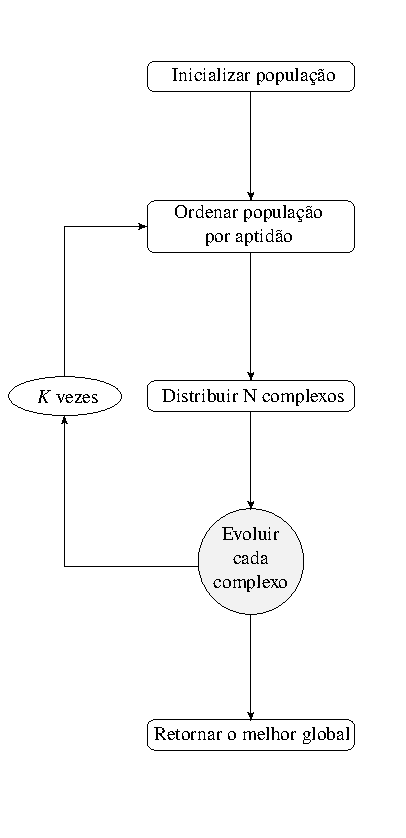
\includegraphics[scale=1.5]{flow1}
  \captionof{figure}{The SCE algorithm overview.}
  \label{fig:flow1}
\end{wrapfigure}

In the SCE a population of $N*M$ individuals is randomly taken from the
feasible solution space.
After this initialization the population is sorted by descending order according
to their fitness and the best global solution is identified.
The entire population is then partitioned (shuffled) into $N$ complexes,
each containing $M$ individuals.
In this shuffling process the first individual goes to the first complex, the second
individual goes to the second complex, individual $N$ goes to $N$-th complex,
individual $M+1$ goes back to the first complex, etc.

\begin{wrapfigure}{L}{0.35\linewidth}
    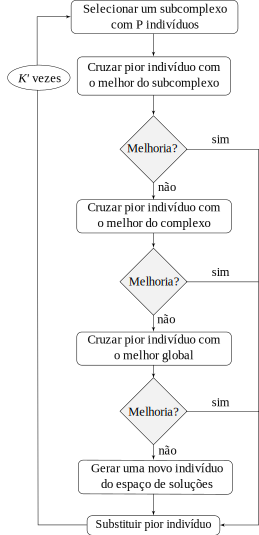
\includegraphics[scale=1.5]{flow2}
  \captionof{figure}{Evolving stage for a single complex.}
  \label{fig:flow2}
\end{wrapfigure}

The next step after shuffling the complexes is to evolve each complex through
a given fixed amount of $K'$ steps.
The individuals in each complex is sorted by descending order of fitness quality.
In each step a subcomplex of $P$ individuals is selected from the
complex using a triangular probability distribution, where the $i$-th individual
has a probability $p_i = \frac{2(n+1-i)}{n(n+1)}$ of being selected.
The use of triangular distribution is intended to prioritize individuals with
better fitness, supporting the algorithm convergence rate.

After the selection of the subcomplex, its worst individual is identified to
be replaced by a new generated solution.
This new solution is generated by the crossing of the worst individual and an
other individual with better fitness.
At first the best individual of the subcomplex is considered for the crossing.
If the new solution is not better than the worst one, the best individual
of the complex is considered for a crossing.
If the latter crossing did not result in any improvement, the best individual
of whole population is considered.
Finally, if all the crossing steps couldn't generate a better individual,
the worst individual of the subcomplex is replaced by a new random solution taken
from the feasible solution space.
This last step is important to prevent the algorithm becoming trapped in local minima.
Fig.~\ref{fig:flow2} presents the evolving procedure described above in a flowchart diagram.

After evolving all the $N$ complexes the whole population is again
sorted by descending order of fitness quality and the process continues until
a stop condition is satisfied.
Fig.~\ref{fig:flow1} shows the SCE algorithm in a flowchart diagram.

\section*{The SCE for the MKP}

As it can be noted in its description the SCE is easly applied to any
optimization problem.
The only steps needed to be specified is (a) the creation of a new random
solution and (b) the crossing procedure of two solutions.
These two procedures are respectively presented by Algorithm.~\ref{alg:new} and
Algorithm~\ref{alg:cross}.

To construct a new random solution (Algorithm~\ref{alg:new}) the items are
at first shuffled in random order and stored in a list (line 2).
A new empty solution is then defined (line 3).
The algorithm iteratively tries to fill the solution's knapsack with 
the an item taken from the list (lines 4-9).
The feasibility of the solution is then checked: if the item insertion let
the solution unfeasible (line 6) its removed from knapsack (line 7).
After trying to place all available items the new solution is returned.

\begin{wrapfigure}{R}{0.50\linewidth}
    
\includegraphics[scale=2]{alg-new}
	\\[1cm]
    
\includegraphics[scale=2]{alg-cross}
  \captionof{figure}{figure caption}
  \label{alg:new}
\end{wrapfigure}

\section*{Computational experiments}

For the computational experiments a batch of tests was driven to find the best
parameters for the problem.
Afterwards two main tests was considered:
(a) using the well-known set of problems defined by Chu and Beasley \cite{Chu-Beasley-1998}
and (b) a large set of randomly generated instances using uniform distribution.

The set of MKP instances provided by Chu and Beasley was generated using a
procedure suggested by Freville and Plateau~\cite{freville1994efficient}, which
attempts to generate instances hard to solve.
The number of constraints $m$ varies among $5$, $10$ and $30$, and the number
of variables $n$ varies among $100$, $250$ and $500$.

\begin{wraptable}{R}{0.6\linewidth}
  \begin{tabular}{|c|c|l|}
  \hline
  \multicolumn{1}{|c}{\rule{0pt}{12pt} \spc } & \multicolumn{1}{|c|}{\bf \spc Value \spc } & \multicolumn{1}{c|}{\bf Description} \\[2pt]
  \hline\rule{0pt}{12pt}
  $N$  & $20$  & \spc \# of complexes \\
  $M$  & $20$  & \spc \# of individuals in each complex \\
  $P$  & $5$   & \spc \# of individuals in each subcomplex \\
  $K$  & $300$ & \spc \# of algorithm iterations \\
  $K'$ & $20$  & \spc \# of iterations of evolving process \\
  $c$  & $n/5$ & \spc \# of genes carried from parent in crossing \\[2pt]
  \hline
  \end{tabular}
  \captionof{table}{Parameters used in SCE algorithm.}
  \label{tab:params}
\end{wraptable}

The $w_{ij}$ were integer numbers drawn from the discrete uniform distribution
$U(0, 1000)$.
The capacity coefficient $c_i$ were set using
$b_i = \alpha\sum_{j=1}^{n} w_{ij}$ where $\alpha$ is a tightness ratio and
varies among $0.25$, $0.5$ and $0.75$.
For each combination of $(m,n,\alpha)$ parameters, $10$ random problems was generated,
totaling $270$ problems.
The profit $p_j$ of the items were correlated to $w_{ij}$ and generated as follows:
\begin{displaymath}
  p_j = \sum_{i=1}^m \frac{w_{ij}}{m} + 500q_j \qquad j = 1, \ldots, n
\end{displaymath}

The second set of instances is composed by problems generated using a similar
setup.
The only differences is that the profit $p_j$ is also drawn from a discrete uniform
distribution $U(0, 1000)$.
For each combination of $(m, n, \alpha)$ parameter, $600$ random problems was
generated, totaling $16200$ problems.

%\subsection{Experimental results}

All the experiments was run on a Intel Core i5-3570 CPU @3.40GHz computer
with 4GB of RAM.
The SCE algorithm for MKP was implemented in C programming language.
For the set of random instance all best known solution was found by the solver
SCIP 3.0.1 running for at least 10 minutes.
SCIP~\cite{achterberg2009scip} is an open-source integer programming solver which
implements the branch-and-cut algorithm~\cite{padberg1991branch}.
\\

\begin{minipage}[t]{0.5\linewidth}
\hspace{3cm}
\begin{tabular}{|r|r|rr|} \hline
\textbf{n}   & \textbf{m}  & \textbf{SCE t (s)} & \textbf{gap (\%)} \\ \hline
   $100$ & $5$  & $0.81$ & $97.6$ \\
	   & $10$ & $0.86$ & $97.0$ \\
	   & $30$ & $1.02$ & $96.7$ \\ \cline{2-4}
    & \multicolumn{2}{r}{{\bf average gap}}  & $\bf 97.1$  \\ \hline
   $250$ & $5$  & $1.75$ & $95.3$ \\
	   & $10$ & $1.83$ & $95.0$ \\
	   & $30$ & $2.24$ & $94.7$ \\ \cline{2-4}
    & \multicolumn{2}{r}{{\bf average gap}}  & $\bf 95.0$  \\ \hline
   $500$ & $5$  & $3.23$ & $93.7$ \\
	   & $10$ & $3.40$ & $93.7$ \\
	   & $30$ & $3.91$ & $93.3$ \\ \cline{2-4}
    & \multicolumn{2}{r}{{\bf average gap}}  & $\bf 93.6$  \\ \hline
\end{tabular}
 \captionof{table}{SCE performance on Chu-Beasley problems.}
 \label{tab:chu}
\end{minipage}
\begin{minipage}[t]{0.5\linewidth}
\centering
\begin{tabular}[c]{|r|r|r|rrr|} \hline
\textbf{n}   & \textbf{m}  & \textbf{$\alpha$}    &\textbf{SCIP t (s)}& \textbf{SCE t (s)} & \textbf{gap (\%)} \\ \hline
$500$ & $10$ & $0.25$ & $278.85$ & $  2.23$  & $96.1$ \\
    &    & $0.50$ & $177.32$ & $  2.14$  & $98.4$ \\
    &    & $0.75$ & $  8.47$ & $  1.87$  & $99.6$ \\ \cline{2-6}
    & \multicolumn{4}{r}{\textbf{average gap}}  & $\bf 98.0$  \\ \hline
    & $20$ & $0.25$ & $284.11$ & $  2.30$  & $96.7$ \\
    &    & $0.50$ & $275.68$ & $  2.16$  & $98.6$ \\
    &    & $0.75$ & $ 33.67$ & $  1.90$  & $99.7$ \\ \cline{2-6}
    & \multicolumn{4}{r}{\textbf{average gap}}  & $\bf 98.3$  \\ \hline
    & $30$ & $0.25$ & $283.78$ & $  2.50$  & $96.9$ \\
    &    & $0.50$ & $283.54$ & $  2.32$  & $98.7$ \\
    &    & $0.75$ & $ 71.66$ & $  1.96$  & $99.7$ \\ \cline{2-6}
    & \multicolumn{4}{r}{\textbf{average gap}}  & $\bf 98.3$  \\ \hline
\end{tabular}
 \captionof{table}{SCE performance on random generated problems.}
 \label{tab:rand}
\end{minipage}

\color{SaddleBrown} % SaddleBrown color for the conclusions to make them stand out

\section*{Conclusions}

In this work we addressed the application of the shuffled complex
evolution (SCE) to the multidimensional knapsack problem and investigated it
performance through several computational experiments.

The SCE algorithm, which combines the ideas of a controlled random search with
the concepts of competitive evolution proved to be very effective in finding
good solution for hard instances of MKP, demanding a very small amount of
processing time to reach high quality solutions for MKP.

\color{DarkSlateGray} % Set the color back to DarkSlateGray for the rest of the content

%----------------------------------------------------------------------------------------
%	FORTHCOMING RESEARCH
%----------------------------------------------------------------------------------------

\section*{Future remarks}

Future work includes the investigation of different crossing procedures,
the use of local search in the process of evolving complexes and the
application of problem reduction procedures for the MKP.


%\nocite{*} % Print all references regardless of whether they were cited in the poster or not
\bibliographystyle{plain} % Plain referencing style
\bibliography{../../../refs} % Use the example bibliography file sample.bib


\section*{Acknowledgements}
Research supported by Funda\c c\~ao de Amparo \`a Pesquisa do Esp\'irito Santo.

\end{multicols}

\end{document}
